\documentclass{standalone}
\usepackage{tikz}
\usetikzlibrary{patterns, positioning}
\usepackage[sfdefault]{ClearSans} %% option 'sfdefault' activates Clear Sans as the default text font
\usepackage[T1]{fontenc}

\begin{document}
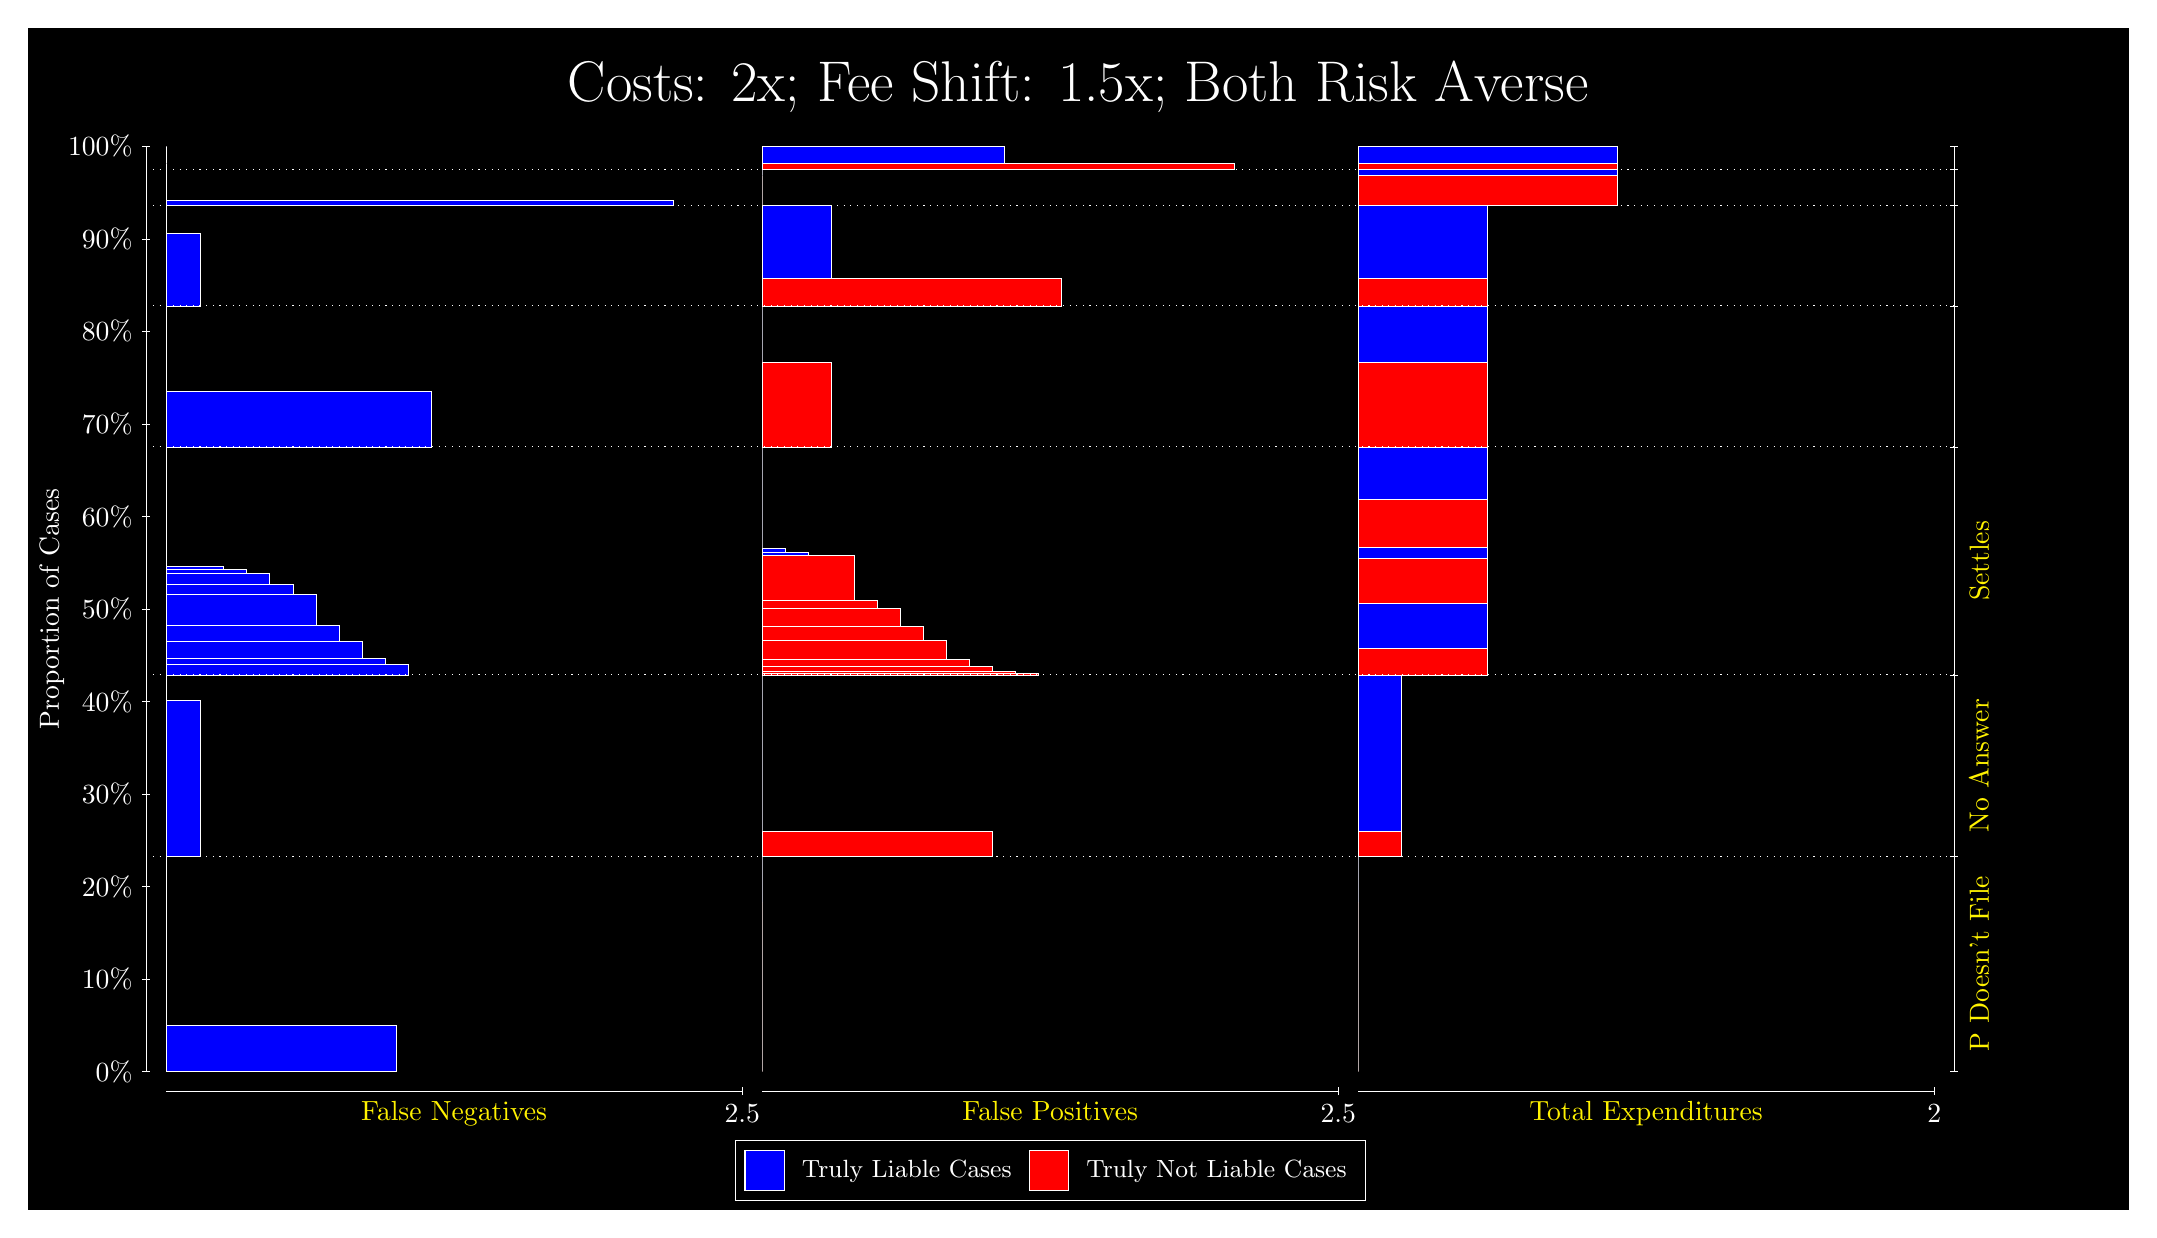
\begin{tikzpicture}
\draw[fill=black] (0,0) rectangle (26.667,15);
\draw[text=white] (0,13.5) rectangle (26.667,15) node[midway] {\huge Costs: 2x; Fee Shift: 1.5x; Both Risk Averse};
\draw[white, very thin] (1.5,1.75) -- (1.5,13.5);
\node[rotate=90, text=white, anchor=center] at (0.3, 7.625) {Proportion of Cases};
\draw[white, very thin] (1.45,1.75) -- (1.55,1.75);
\node[text=white, anchor=east] at (1.45, 1.75) {0\%};
\draw[white, very thin] (1.45,2.925) -- (1.55,2.925);
\node[text=white, anchor=east] at (1.45, 2.925) {10\%};
\draw[white, very thin] (1.45,4.1) -- (1.55,4.1);
\node[text=white, anchor=east] at (1.45, 4.1) {20\%};
\draw[white, very thin] (1.45,5.275) -- (1.55,5.275);
\node[text=white, anchor=east] at (1.45, 5.275) {30\%};
\draw[white, very thin] (1.45,6.45) -- (1.55,6.45);
\node[text=white, anchor=east] at (1.45, 6.45) {40\%};
\draw[white, very thin] (1.45,7.625) -- (1.55,7.625);
\node[text=white, anchor=east] at (1.45, 7.625) {50\%};
\draw[white, very thin] (1.45,8.8) -- (1.55,8.8);
\node[text=white, anchor=east] at (1.45, 8.8) {60\%};
\draw[white, very thin] (1.45,9.975) -- (1.55,9.975);
\node[text=white, anchor=east] at (1.45, 9.975) {70\%};
\draw[white, very thin] (1.45,11.15) -- (1.55,11.15);
\node[text=white, anchor=east] at (1.45, 11.15) {80\%};
\draw[white, very thin] (1.45,12.325) -- (1.55,12.325);
\node[text=white, anchor=east] at (1.45, 12.325) {90\%};
\draw[white, very thin] (1.45,13.5) -- (1.55,13.5);
\node[text=white, anchor=east] at (1.45, 13.5) {100\%};

\draw[white, very thin] (24.457,1.75) -- (24.457,13.5);
\draw[white, very thin] (24.407,1.75) -- (24.507,1.75);
\node[anchor=west] at (24.407, 1.75) {};
\draw[white, very thin] (24.407,4.4851) -- (24.507,4.4851);
\node[anchor=west] at (24.407, 4.4851) {};
\draw[white, very thin] (24.407,6.7868) -- (24.507,6.7868);
\node[anchor=west] at (24.407, 6.7868) {};
\draw[white, very thin] (24.407,9.6824) -- (24.507,9.6824);
\node[anchor=west] at (24.407, 9.6824) {};
\draw[white, very thin] (24.407,11.473) -- (24.507,11.473);
\node[anchor=west] at (24.407, 11.473) {};
\draw[white, very thin] (24.407,12.745) -- (24.507,12.745);
\node[anchor=west] at (24.407, 12.745) {};
\draw[white, very thin] (24.407,13.208) -- (24.507,13.208);
\node[anchor=west] at (24.407, 13.208) {};
\draw[white, very thin] (24.407,13.5) -- (24.507,13.5);
\node[anchor=west] at (24.407, 13.5) {};

\draw[white, very thin, fill=blue] (1.75,1.75) rectangle (4.6775,2.3331);
\draw[white, very thin, fill=red] (1.75,2.3331) rectangle (1.75,4.4851);
\draw[white, very thin, fill=blue] (1.75,4.4851) rectangle (2.1891,6.47);
\draw[white, very thin, fill=red] (1.75,6.47) rectangle (1.75,6.7868);
\draw[white, very thin, fill=blue] (1.75,6.7868) rectangle (4.8239,6.9226);
\draw[white, very thin, fill=blue] (1.75,6.9226) rectangle (4.5312,6.9931);
\draw[white, very thin, fill=blue] (1.75,6.9931) rectangle (4.2384,7.2174);
\draw[white, very thin, fill=blue] (1.75,7.2174) rectangle (3.9457,7.4237);
\draw[white, very thin, fill=blue] (1.75,7.4237) rectangle (3.6529,7.814);
\draw[white, very thin, fill=blue] (1.75,7.814) rectangle (3.3602,7.9383);
\draw[white, very thin, fill=blue] (1.75,7.9383) rectangle (3.0674,8.0743);
\draw[white, very thin, fill=blue] (1.75,8.0743) rectangle (2.7746,8.1238);
\draw[white, very thin, fill=blue] (1.75,8.1238) rectangle (2.4819,8.1637);
\draw[white, very thin, fill=red] (1.75,8.1637) rectangle (1.75,9.6824);
\draw[white, very thin, fill=blue] (1.75,9.6824) rectangle (5.1167,10.395);
\draw[white, very thin, fill=red] (1.75,10.395) rectangle (1.75,11.473);
\draw[white, very thin, fill=blue] (1.75,11.473) rectangle (2.1891,12.398);
\draw[white, very thin, fill=red] (1.75,12.398) rectangle (1.75,12.745);
\draw[white, very thin, fill=blue] (1.75,12.745) rectangle (8.1906,12.82);
\draw[white, very thin, fill=red] (1.75,12.82) rectangle (1.75,13.208);
\draw[white, very thin, fill=red] (1.75,13.208) rectangle (1.75,13.283);
\draw[white, very thin, fill=blue] (1.75,13.283) rectangle (1.75,13.5);
\draw[white, very thin, fill=red] (9.3189,1.75) rectangle (9.3189,3.902);
\draw[white, very thin, fill=blue] (9.3189,3.902) rectangle (9.3189,4.4851);
\draw[white, very thin, fill=red] (9.3189,4.4851) rectangle (12.246,4.8019);
\draw[white, very thin, fill=blue] (9.3189,4.8019) rectangle (9.3189,6.7868);
\draw[white, very thin, fill=red] (9.3189,6.7868) rectangle (12.832,6.8057);
\draw[white, very thin, fill=red] (9.3189,6.8057) rectangle (12.539,6.829);
\draw[white, very thin, fill=red] (9.3189,6.829) rectangle (12.246,6.8983);
\draw[white, very thin, fill=red] (9.3189,6.8983) rectangle (11.954,6.9822);
\draw[white, very thin, fill=red] (9.3189,6.9822) rectangle (11.661,7.2286);
\draw[white, very thin, fill=red] (9.3189,7.2286) rectangle (11.368,7.3993);
\draw[white, very thin, fill=red] (9.3189,7.3993) rectangle (11.075,7.6298);
\draw[white, very thin, fill=red] (9.3189,7.6298) rectangle (10.783,7.7369);
\draw[white, very thin, fill=red] (9.3189,7.7369) rectangle (10.49,8.3056);
\draw[white, very thin, fill=blue] (9.3189,8.3056) rectangle (9.9044,8.3454);
\draw[white, very thin, fill=blue] (9.3189,8.3454) rectangle (9.6116,8.3949);
\draw[white, very thin, fill=blue] (9.3189,8.3949) rectangle (9.3189,9.6824);
\draw[white, very thin, fill=red] (9.3189,9.6824) rectangle (10.197,10.761);
\draw[white, very thin, fill=blue] (9.3189,10.761) rectangle (9.3189,11.473);
\draw[white, very thin, fill=red] (9.3189,11.473) rectangle (13.125,11.82);
\draw[white, very thin, fill=blue] (9.3189,11.82) rectangle (10.197,12.745);
\draw[white, very thin, fill=red] (9.3189,12.745) rectangle (9.3189,13.132);
\draw[white, very thin, fill=blue] (9.3189,13.132) rectangle (9.3189,13.208);
\draw[white, very thin, fill=red] (9.3189,13.208) rectangle (15.32,13.283);
\draw[white, very thin, fill=blue] (9.3189,13.283) rectangle (12.393,13.5);
\draw[white, very thin, fill=red] (16.888,1.75) rectangle (16.888,3.902);
\draw[white, very thin, fill=blue] (16.888,3.902) rectangle (16.888,4.4851);
\draw[white, very thin, fill=red] (16.888,4.4851) rectangle (17.437,4.8019);
\draw[white, very thin, fill=blue] (16.888,4.8019) rectangle (17.437,6.7868);
\draw[white, very thin, fill=red] (16.888,6.7868) rectangle (18.534,7.1258);
\draw[white, very thin, fill=blue] (16.888,7.1258) rectangle (18.534,7.7016);
\draw[white, very thin, fill=red] (16.888,7.7016) rectangle (18.534,8.2702);
\draw[white, very thin, fill=blue] (16.888,8.2702) rectangle (18.534,8.406);
\draw[white, very thin, fill=red] (16.888,8.406) rectangle (18.534,9.0172);
\draw[white, very thin, fill=blue] (16.888,9.0172) rectangle (18.534,9.6824);
\draw[white, very thin, fill=red] (16.888,9.6824) rectangle (18.534,10.761);
\draw[white, very thin, fill=blue] (16.888,10.761) rectangle (18.534,11.473);
\draw[white, very thin, fill=red] (16.888,11.473) rectangle (18.534,11.82);
\draw[white, very thin, fill=blue] (16.888,11.82) rectangle (18.534,12.745);
\draw[white, very thin, fill=red] (16.888,12.745) rectangle (20.181,13.132);
\draw[white, very thin, fill=blue] (16.888,13.132) rectangle (20.181,13.208);
\draw[white, very thin, fill=red] (16.888,13.208) rectangle (20.181,13.283);
\draw[white, very thin, fill=blue] (16.888,13.283) rectangle (20.181,13.5);
\draw[white, dotted] (1.5,4.4851) -- (24.457,4.4851);
\draw[white, dotted] (1.5,6.7868) -- (24.457,6.7868);
\draw[white, dotted] (1.5,9.6824) -- (24.457,9.6824);
\draw[white, dotted] (1.5,11.473) -- (24.457,11.473);
\draw[white, dotted] (1.5,12.745) -- (24.457,12.745);
\draw[white, dotted] (1.5,13.208) -- (24.457,13.208);
\draw[white, very thin] (1.75,1.5) -- (9.0689,1.5);
\node[text=yellow, anchor=north] at (5.4094, 1.5) {False Negatives};
\draw[white, very thin] (9.0689,1.45) -- (9.0689,1.55);
\node[text=white, anchor=north] at (9.0689, 1.45) {2.5};

\draw[white, very thin] (9.3189,1.5) -- (16.638,1.5);
\node[text=yellow, anchor=north] at (12.978, 1.5) {False Positives};
\draw[white, very thin] (16.638,1.45) -- (16.638,1.55);
\node[text=white, anchor=north] at (16.638, 1.45) {2.5};

\draw[white, very thin] (16.888,1.5) -- (24.207,1.5);
\node[text=yellow, anchor=north] at (20.547, 1.5) {Total Expenditures};
\draw[white, very thin] (24.207,1.45) -- (24.207,1.55);
\node[text=white, anchor=north] at (24.207, 1.45) {2};

\node[text=yellow, centered, rotate=90] at (24.777, 3.1176) {P Doesn't File};
\node[text=yellow, centered, rotate=90] at (24.777, 5.636) {No Answer};
\node[text=yellow, centered, rotate=90] at (24.777, 8.2346) {Settles};





\draw (12.978300999999998,1.5) node[draw=none] (baseCoordinate) {};
\begin{scope}[align=center]
        \matrix[scale=0.5, draw=white, below=0.5cm of baseCoordinate, nodes={draw}, column sep=0.1cm]{
            \node[rectangle, draw, minimum width=0.5cm, minimum height=0.5cm, fill=blue] {}; &
            \node[draw=none, font=\small, text=white] (B) {Truly Liable Cases}; &
            \node[rectangle, draw, minimum width=0.5cm, minimum height=0.5cm, fill=red] {}; &
            \node[draw=none, font=\small, text=white] (B) {Truly Not Liable Cases}; \\
            };
\end{scope}

\end{tikzpicture}
\end{document}